\section{Memory Provenance as Persistent Agent State}
\label{sec:formulation}
Consider an acquisition episode with task $x$ and trajectory $\tau$. Its terminal outcome is $z\in\{0,1\}$. A memory writer receives the episode and produces a textual memory
\begin{equation}
M = G(\tau, z).
\end{equation}
ReasoningBank instantiates $G$ with outcome-conditioned reflection. The successful branch asks the writer to explain the strategy that worked. The failure branch asks the writer to identify the cause of failure and construct an improved approach. We call the branch variable $P\in\{S,F\}$ the memory provenance.

A future query $x'$ retrieves a memory through a similarity function $R(x',x)$. The retrieval key can be identical even when the written memory differs because the key is the historical task description. Future behavior then follows
\begin{equation}
Y = H(x',M(P),S),
\end{equation}
where $S$ denotes the rest of the agent state. Provenance reaches future behavior through memory content. It is therefore an upstream causal variable with direct influence on the persistent state.

\begin{figure}[t]
\centering
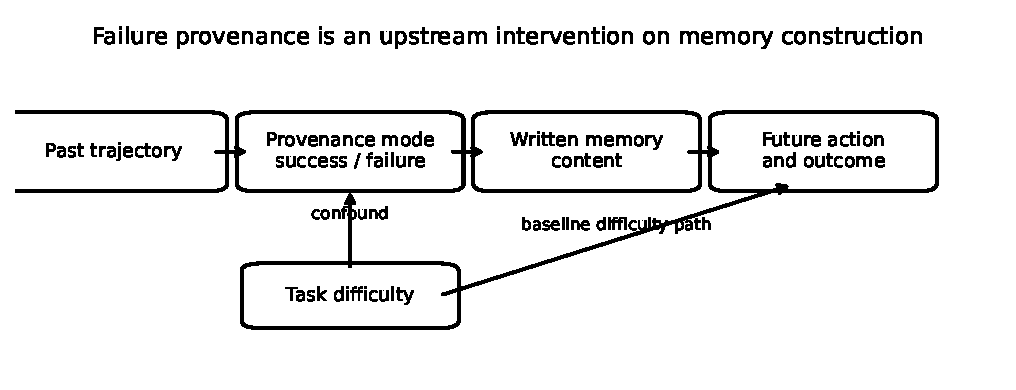
\includegraphics[width=\linewidth]{figures/fig1_provenance_causal.pdf}
\caption{Causal structure of provenance-conditioned memory. Task difficulty affects which trajectories fail and also affects future outcomes. The matched-memory intervention blocks this confound by fixing the future query and matching semantic guidance across provenance conditions.}
\label{fig:causal}
\end{figure}

\subsection{Target estimand}
Let $C(M)$ denote the semantic guidance contained in a memory. The quantity of interest is the effect of provenance under matched guidance:
\begin{equation}
\Delta_{P}(x')=
\mathbb{E}[Y\mid do(P=F),C(M)=c,x']-
\mathbb{E}[Y\mid do(P=S),C(M)=c,x'].
\label{eq:effect}
\end{equation}
For a success indicator, a negative $\Delta_P$ means failure provenance reduces future success under matched information. For an error indicator, the sign reverses.

Task difficulty $D$ creates the central identification challenge. Difficult acquisition tasks yield more failed trajectories. They also remain difficult when encountered later. Conditioning only on observed provenance therefore estimates a mixture of provenance effect and task difficulty. Equation~\ref{eq:effect} motivates a direct intervention on the retrieved memory while the future task remains fixed.

\subsection{Matched provenance pairs}
A provenance pair contains two memories with the same intended procedural guidance. One member is derived from a successful trajectory. The other member is derived from a failed trajectory. Matching is performed over the task family and the actionable recommendation. Each pair is checked for information asymmetry before it enters the experiment. A pair is rejected when one memory contains an extra fact that can independently solve the future task.

This construction turns provenance into an experimentally manipulable state variable. It also exposes a design principle for memory systems: a textual memory is incomplete as an audit object when its learning process has been discarded. Provenance metadata preserves evidence about whether the remembered strategy emerged from demonstrated success or from a corrective interpretation of failure.
